\documentclass[12pt, a4paper, oneside]{ctexart}
\usepackage{amsmath, amsthm, amssymb, bm, color, framed, graphicx, hyperref, mathrsfs, mathtools, enumerate, tikz}
\usetikzlibrary{patterns}

\title{\textbf{Homework 2}}
\author{王一鑫\quad 作业序号42}
\date{\today}
\linespread{1.5}
\newcounter{problemname}
\newenvironment{problem}{\begin{framed}\stepcounter{problemname}\par\noindent\textsc{Problem \arabic{problemname}. }}{\end{framed}\par}
\newenvironment{solution}{%
	\par\noindent\textsc{Solution. }\ignorespaces
}{%
	\hfill$\qed$\par
}
\newenvironment{note}{\par\noindent\textsc{Note of Problem \arabic{problemname}. }}{\\\par}

\begin{document}
	
	\maketitle
	
	\begin{problem}
		\textbf{Weierstrass' calssical counterexample from 1870.} Consider the minimum problem\[ F(u)\coloneqq\int_{-1}^{1}(xu^{\prime}(x))^{2}\mathrm{d}x = \min!\quad u\in C^{1}[-1,1]\quad u(-1)=0\quad u(1)=1\]Use the sequence \[ u_{n}(x)\coloneqq\dfrac{1}{2}+\dfrac{1}{2}\dfrac{\arctan nx}{\arctan n}\quad n=1,2,\cdots \]in order to show that this variational problem has \textbf{no solution}. Recall that $C^{1}[-1,1]$ denotes the space of continuously differentiable functions $u:[-1,1]\rightarrow\mathbb{R}$.
	\end{problem}
	\begin{solution}
		Set $M\equiv\{u\in C^{1}[-1,1]: u(-1)=0\ \text{and } u(1) = 1\}$. Then, the problem is equivalent to\[ F(u)=\min!\quad u\in M \] Since $u_{n}(-1) = 0$ and $u_{n}(1)=1$, we get $u_{n}\in M$ for all $n$. We calculate
		\begin{align*}
			F(u_{n}) = \int_{-1}^{1}(xu_{n}^{\prime}(x))^{2}\mathrm{d}x&\leq\int_{-1}^{1}(x^{2}+\dfrac{1}{n^{2}})(u_{n}^{\prime}(x))^{2}\mathrm{d}x\\&= \dfrac{1}{4(\arctan n)^{2}}\int_{-1}^{1}\dfrac{1+n^{2}x^{2}}{n^{2}}\cdot\dfrac{n^{2}}{(1+n^{2}x^{2})^{2}}\mathrm{d}x\\&=\dfrac{1}{4(\arctan n)^{2}}\int_{-n}^{n}\dfrac{\mathrm{d}y}{1+y^{2}}\\&=\dfrac{1}{2n\cdot\arctan n}
		\end{align*}
		Hence, $F(u_{n})\rightarrow0$ as $n\rightarrow\infty$. Since $F(u)\geq0$ for all $u\in M$, this implies \[ \mathop{inf}\limits_{u\in M}F(u) = 0 \]
		
		Suppose now that $u$ is a solution of the minimum problem. Then\[ F(u) = 0\quad u \in M \]and hence \[ xu^{\prime}(x) =  0\quad\text{for all }x\in [-1,1] \] This implies $u^{\prime}(x) = 0$ on $[-1,1]$, i.e., $u(x) =$ const. But this contradicts with the side condition $u(-1)=0$ and $u(1) = 1$.
	\end{solution}
	
	\begin{note}
		This example was given by Weierstrass to show that a minimum problem in the calculus of variations need not always have a solution, namely.
		
		The infimum of the functional $F$ on the set $M$ is not attained at some point $u$ of $M$.
	\end{note}
	
	\begin{problem}
		\textbf{The classical Hilbert space $l_{2}^{\mathbb{K}}$}. By definition, the space $l_{2}^{\mathbb{K}}$ consists of all the seqences $(u_{n})_{n\geq1}$ with $u_{n}\in\mathbb{K}$ for all $n\in\mathbb{N}$ and \[ \sum_{n=1}^{\infty}|u_{n}|^{2}<\infty \]Show that $l_{2}^{\mathbb{K}}$ is an infinite-dimensional Hilbert space over $\mathbb{K}$ equipped with the inner product\[ \langle u ,v \rangle\coloneqq\sum_{n=1}^{\infty}\bar{u}_{n}v_{n} \]where $u\coloneqq(u_{n})$ and $v\coloneqq(v_{n})$.
	\end{problem}
	\begin{solution}
		We have shown $l_{2}^{\mathbb{K}}$ is a infinite-dimensional linear space over $\mathbb{K}$.
		
		\textbf{Step 1}: Show that $\langle\ ,\ \rangle$ is an inner product.
		\begin{enumerate}[(1)]
			\item For any $u\in l_{2}^{\mathbb{K}}$, we have \[ \langle u, u\rangle = \sum_{n=1}^{\infty}\bar{u}_{n}u_{n} = \sum_{n=1}^{\infty}|u_{n}|^{2}\geq0\]and $\langle u,u\rangle = 0$ iff $u_{n} = 0$ for each $n=1,2,\cdots$, that is, $u=0$.
			\item For any $u,v,w\in l_{2}^{\mathbb{K}}$, and $\alpha, \beta\in\mathbb{K}$, we have \begin{align*}
				\langle u, \alpha v + \beta w\rangle &= \sum_{n=1}^{\infty}\bar{u}_{n}(\alpha v_{n+\beta w_{n}}) \\&= \alpha\sum_{n=1}^{\infty}\bar{u}_{n}v_{n} + \beta\sum_{n=1}^{\infty}\bar{u}_{n}w_{n}\\&=\alpha\langle u,v\rangle + \beta \langle u, w\rangle
			\end{align*}  
			\item For any $u,v\in l_{2}^{\mathbb{K}}$\[ \overline{\langle u,v\rangle} = \overline{\sum_{n=1}^{\infty}\bar{u}_{n}v_{n}} = \sum_{n=1}^{\infty}\bar{v}_{n}u_{n}=\langle v,u\rangle \]
		\end{enumerate}
		 Choose a Cauchy sequence $(u_{n}^{(k)})$ in $l_{2}^{\mathbb{K}}$, which means for $\forall\varepsilon>0$, there exists $N>0$, such that $\forall k_{1}, k_{2}\geq N$, we have \begin{align*}
		 	\Vert (u_{n}^{(k_{1})}-u_{n}^{(k_{2})})\Vert&=\langle u^{k_{1}}-u^{k_{2}},u^{k_{1}}-u^{k_{2}}\rangle^{\frac{1}{2}}\\&=\Big(\sum_{n=1}^{\infty}|u_{n}^{(k_{1})}-u_{n}^{(k_{2})}|^{2}\Big)^{\frac{1}{2}}<\varepsilon
		 \end{align*}  
		 Since \[ |u_{n}^{(k_{1})}-u_{n}^{(k_{2})}| < \Vert (u_{n}^{(k_{1})}-u_{n}^{(k_{2})})\Vert<\varepsilon\quad\text{for every } n \]
		 By applying the classical Cauchy convergence theorem, $u_{n}^{(k)}$ converges to $u_{n}^{*}$ and $u^{*} = (u_{n}^{*})$. It suffices to show that $u^{*}\in l_{2}^{\mathbb{K}}$ and $\|u^{(k)}-u^{*}\|\to0$.
%		 Apply the limiting process $N\to\infty$ to the classical Schwarz inequality\[ \left| \sum_{n=1}^N \overline{u}_{n} v_n \right| \leq \left( \sum_{n=1}^N |u_n|^2 \right)^{\frac{1}{2}} \left( \sum_{n=1}^N |v_n|^2 \right)^{\frac{1}{2}} \]We get \[ \left|\sum_{n=1}^{\infty}\big(u_{n}^{(k_{1})}-u_{n}^{(k_{2})}\big)\right|\leq\Big(\sum_{n=1}^{\infty}|u_{n}^{(k_{1})}-u_{n}^{(k_{2})}|^{2}\Big)^{\frac{1}{2}}\Big(\sum_{n=1}^{\infty}1\Big)^{\frac{1}{2}}<\varepsilon \]
		Restricting the summation to $n\leq N$ and letting $k_{2}\to\infty$, we obtain\[ \Big(\sum_{n=1}^{N}|u_{n}^{(k_{1})}-u_{n}^{*}|^{2}\Big)^{\frac{1}{2}}<\varepsilon \]Letting $N\to\infty$, we get \[ \|u^{(k_{1})} - u^{*}\|<\varepsilon \]That is, $\|u^{(k)}-u^{*}\|\to0$. and \[ \|u^{*}\|\leq\|u^{*}-u^{(k)}\| + \|u^{(k)}\| \in l_{2}^{\mathbb{K}}  \]
	\end{solution}
	\begin{problem}
		\textbf{The Banach space \( C[a,b] \)} Let \( -\infty < a < b < \infty \). Show that the Banach space \( C[a, b] \) equipped with the usual maximum norm 
		\[
		\|u\| = \max_{a \leq x \leq b} |u(x)|
		\]
		is \textit{not} a Hilbert space.
	\end{problem}
	
	\begin{solution}
		Suppose it is a Hilbert space, then the \textbf{parallelogram identity} holds:\[ 2\|u\|^{2}+2\|v\|^{2} = \|u+v\|^{2} + \|u-v\|^{2}\quad \forall u, v\in C[a,b] \]However
		\begin{align*}
			 \|u+v\|^{2} + \|u-v\|^{2} &= \max_{a \leq x \leq b}|u(x)+v(x)| + \max_{a \leq x \leq b}|u(x)-v(x)| \\&\leq 2\max_{a \leq x \leq b}|u(x)| + 2\max_{a \leq x \leq b}|v(x)| = 2\|u\|^{2} + 2\|v\|^{2} 
		\end{align*}
		Thus the parallelogram identity is violated.
	\end{solution}
	
	\begin{problem}
		 \textbf{The Ritz method.}
			By Section 2.7.1, the variational problem
			\[
			\int_0^{\pi} \left( 2^{-1} u'^2 - u \cos x \right) dx = \min !, \quad u \in C^2[0, \pi], \quad u(0) = u(\pi) = 0 \tag{V}
			\]
			is equivalent to the boundary-value problem
			\[
			u''(x) + \cos x = 0 \quad \text{on } [0, \pi], \quad u(0) = u(\pi) = 0, \tag{B}
			\]
			which has a unique solution \( u \). Explicitly,
			\[
			u(x) = \cos x + 2\pi^{-1} x - 1.
			\]
			
			Use the Ritz method in order to compute an approximate solution \( u_{2n} \) of (V), by making the ansatz
			\[
			u_{2n}(x) = \sum_{k=1}^{2n} c_k \sin kx.
			\]
			Determine the coefficients \( c_1, \dots, c_{2n} \). Show that \( (u_{2n}) \) converges uniformly on \( [0, \pi] \) to the solution \( u \) of (V).
		
	\end{problem}
	
	\begin{solution}
		The Ritz method yields an approximate solution\[ u_{2n}(x) = \sum_{k=1}^{2n}c_{k}\sin kx \]where the unknown coefficients $c_{k}$ are determined by the minimum problem\[ F(c)\coloneqq\int_{0}^{\pi}(2^{-1}u_{2n}^{\prime\, 2} - u_{2n}\cos x)\mathrm{d}x = \min ! \]
		We compute\[ u_{2n}^{\prime} = \sum_{k=1}^{2n}kc_{k}\cos kx \]and\[ F(c) = \int_{0}^{\pi}\big(\dfrac{1}{2}(\sum_{k=1}^{2n}kc_{k}\cos kx)^{2}- \sum_{k=1}^{2n}c_{k}\sin kx\cos x\big)\mathrm{d}x\]To solve the minimum problem, we set derivative with respect to each $c_{k}$\[ \dfrac{\partial F}{\partial c_{k}} = 0 \] So
		\begin{align*}
			\dfrac{\partial F}{\partial c_{k}}&=\int_{0}^{\pi}\big((\sum_{j=1}^{2n}jc_{j}\cos jx)\cdot k\cos kx-\sin kx\cos x\big)\mathrm{d}x\\&=
			\begin{cases}
				\int_{0}^{\pi}k^{2}c_{k}\cos^{2} kx\mathrm{d}x - \dfrac{2k}{k^{2}-1} & k\text{ even}\\
				\int_{0}^{\pi}k^{2}c_{k}\cos^{2} kx\mathrm{d}x - 0 & k\text{ odd}
			\end{cases}\\
			& = \begin{cases}
				\dfrac{\pi k^{2}}{2} c_{k} - \dfrac{2k}{k^{2}-1} & k\text{ even}\\
				\dfrac{\pi k^{2}}{2} c_{k} - 0 & k\text{ odd}
			\end{cases}
		\end{align*}
		Thus we determine the coefficients $c_{k}$\[ c_{k} = \begin{cases}
			 \dfrac{2}{\pi}\cdot\dfrac{1}{r(4r^{2}-1)} & k = 2r\\
		 0 & k = 2r-1
		\end{cases} \]
		That is ,\[ u_{2n} = \dfrac{2}{\pi}\sum_{r=1}^{n}\dfrac{\sin 2rx}{r(4r^{2}-1)} \]As $n\to\infty$, this series converges uniformly on $[0,\pi]$ to the exact solution $u(x)= \cos x-2\pi^{-1}x-1$ by the convergence of Ritz method.
	\end{solution}
	
	Before moving on to the next problem, we introduce an important \textit{smoothing technique} first.
	
	\noindent \textbf{Smoothing of functions by using mean values (Friedrichs' mollification).} The point of departure is the integral
	\[
	u_\varepsilon(x) := \int_{\mathbb{R}^N} \phi_\varepsilon(x - y) u(y) \, dy,
	\]
	where \( \phi_\varepsilon(x) := \varepsilon^{-N} \phi(\varepsilon^{-1} x) \) along with
	\[
	\phi(x) := 
	\begin{cases} 
		ce^{-(1 - |x|^2)^{-1}} & \text{if } x \in \mathbb{R}^N \text{ and } |x| < 1, \\
		0 & \text{if } x \in \mathbb{R}^N \text{ and } |x| \geq 1.
	\end{cases}
	\]
	
	Then
	\begin{itemize}
		\item[(i)] \( \phi \in C_0^{\infty}(\mathbb{R}^N) \).
		\item[(ii)] \( \phi \geq 0 \) on \( \mathbb{R}^N \).
		\item[(iii)] \( \int_{\mathbb{R}^N} \phi(x) \, dx = 1 \) for a suitable choice of the constant \( c > 0 \).
	\end{itemize}
	
	\noindent Hence:
	\begin{itemize}
		\item[(i*)] \( \phi_\varepsilon \in C_0^{\infty}(\mathbb{R}^N) \) and \( \phi_\varepsilon(x) = 0 \) if \( |x| \geq \varepsilon \) for all \( \varepsilon > 0 \).
		\item[(ii*)] \( \phi_\varepsilon \geq 0 \) on \( \mathbb{R}^N \) for all \( \varepsilon > 0 \).
		\item[(iii*)] \( \int_{\mathbb{R}^N} \phi_\varepsilon(x) \, dx = 1 \) (see Figure 2.17 for \( N = 1 \)).
	\end{itemize}
	
	\noindent Let \( u \in L_2(G) \), where \( G \) is a nonempty open set in \( \mathbb{R}^N \), \( N \geq 1 \). We set \( u(x) = 0 \) outside \( G \). Then
	\begin{itemize}
		\item[(\(\alpha\))] \( u_\varepsilon \in C^{\infty}(\mathbb{R}^N) \) for all \( \varepsilon > 0 \).
		\item[(\(\beta\))] \( u_\varepsilon \in L_2(G) \) for all \( \varepsilon > 0 \).
		\item[(\(\gamma\))] \( u_\varepsilon \to u \) in \( L_2(G) \) as \( \varepsilon \to +0 \).
	\end{itemize}
	Now we will use the technique to show the following problems.
	\begin{problem}
		\textbf{Density}
		(Proof of Proposition 7 in Section 2.2). Let \( G \) be a nonempty open set in \( \mathbb{R}^N \), \( N \geq 1 \).
		\begin{enumerate}[(a)]
			\item  Show that the set \( C^{\infty}(G) \) is \textit{dense} in \( L_2(G) \). 
			
			\item  Show that \( C^{\infty}_0(G) \) is \textit{dense} in \( L_2(G) \).
			
			\item  Show that \( C(\overline{G}) \) is \textit{dense} in \( L_2(G) \).
		\end{enumerate}
	\end{problem}
	
	\begin{solution}
		\begin{enumerate}[(a)]
			\item \textsc{Solution:} \textbf{Step 1}: First we show $u_{\varepsilon}\in C^{\infty}(G)$. Consider the ball
			\[
			B := \{x \in G\subseteq\mathbb{R}^N : |x - x_0| < 1\}
			\]
			around the given point \( x_0 \), and consider the set
			\[
			B_\varepsilon := \{y \in G : \text{dist}(B, y) \leq \varepsilon\}.
			\]
			Since \( \phi_\varepsilon(x - y) = 0 \) for all points \( x, y \in \mathbb{R}^N \) with \( |x - y| \geq \varepsilon \)
			\[
			u_\varepsilon(x) = \int_{B_\varepsilon} \phi_\varepsilon(x - y) u(y) \, dy \quad \text{for all } x \in B.
			\]
			
			By the \textit{Schwarz inequality}, we obtain
			\[
			\int_{B_\varepsilon} |u(y)| \, dy = \int_{B_\varepsilon} 1 \cdot |u(y)| \, dy \leq \left( \int_{B_\varepsilon} \, dy \right)^{\frac{1}{2}} \left( \int_{B_\varepsilon} |u(y)|^2 \, dy \right)^{\frac{1}{2}} < \infty,
			\]
			since \( \int_{B_\varepsilon} \, dy = |B_\varepsilon| < \infty \) and \( u \in L_2(G) \) implies \( u \in L_{2}(B_\varepsilon) \). Thus, $u\in L(B_\varepsilon)$ .
			
			First let \( N = 1 \). For all \( x \in B \), \( y \in B_\varepsilon \), and \( k = 0, 1, 2, \ldots \), \( \varepsilon > 0 \), we obtain
			\[
			\left| \phi_\varepsilon^{(k)}(x - y) u(y) \right| \leq \text{const}(k, \varepsilon) |u(y)|, \tag{114}
			\]
			where \( \phi_\varepsilon^{(k)} \) denotes the \( k \)-th derivative. In this connection, note that the function \( \phi_\varepsilon^{(k)} \) is continuous on \( \mathbb{R} \), and hence it is bounded on compact sets by the Weierstrass theorem. In particular, \( \phi_\varepsilon^{(k)} \) is bounded on each ball.
			
			Applying standard theorems on parameter integrals, the continuous derivative \( u_\varepsilon^{(k)} \) exists on \( B \), where
			\[
			u_\varepsilon^{(k)}(x) := \int_{B_\varepsilon} \phi_\varepsilon^{(k)}(x - y) u(y) \, dy \quad \text{for all } x \in B, \quad k = 0, 1, \ldots.
			\]Since the center $x_{0}$ of the ball $B$ is arbitrary, this implies $u_{\varepsilon}\in C^{\infty}(G)$.
			
			\textbf{Step 2}: We show $u_{\varepsilon}\to u$ in $L_{2}(G)$ as $\varepsilon\to+0$. 
			
			Let \( B := \{z \in \mathbb{R}^N : |z| < 1\} \). Recall that \( \phi = 0 \) outside and \( \int_B \phi(z) \, dz = 1 \). Set $z = \varepsilon^{-1}(x-y)$, we have
			\[
			u_\varepsilon(x) = \int_B u(x - \varepsilon z) \phi(z) \, dz,
			\]
			and hence
			\[
			u_\varepsilon(x) - u(x) = \int_B (u(x - \varepsilon z) - u(x)) \phi(z) \, dz.
			\]
			
			The \textit{Schwarz inequality} yields
			\begin{align*}
				|u_\varepsilon(x) - u(x)|^2 &=|\int_B (u(x - \varepsilon z) - u(x)) \phi(z) \, dz|^{2}\\&\leq C \int_B |u(x - \varepsilon z) - u(x)|^2 \, dz
			\end{align*}
			
			
			
			where \( C \) is a positive constant. By the \textit{p-mean continuity} of the Lebesgue integral with \( p = 2 \), for each \( \eta \), there is an \( \varepsilon_0 > 0 \) such that
			\[
			\int_G |u(x - \varepsilon z) - u(x)|^2 \, dx < \eta
			\]
			for all \( z \in B \) and all \( \varepsilon : 0 < \varepsilon \leq \varepsilon_0 \). Thus, it follows from the \textit{Fubini–Tonelli theorem} that
			\begin{align*}
				\int_G |u_\varepsilon(x) - u(x)|^2 \, dx &\leq C \int_G \left( \int_B |u(x - \varepsilon z) - u(x)|^2 \, dz \right) dx\\
				&= C \left( \int_B \int_G |u(x - \varepsilon z) - u(x)|^2 \, dx \right) dz \\&\leq C \, |B| \cdot \eta
			\end{align*}
			
			
			for all \( \varepsilon : 0 < \varepsilon \leq \varepsilon_0 \). Hence
			\[
			\int_G |u_\varepsilon(x) - u(x)|^2 \, dx \to 0 \quad \text{as } \varepsilon \to +0.
			\]
			
			This is $u_{\varepsilon}\to u$ in $L_{2}(G)$ as $\varepsilon\to+0$.
			
			Therefore, $C^{\infty}(G)$ is dense in $L_{2}(G)$.
			
			\item 
			\textbf{ Case A}: The nonempty open set \( G \) is bounded. Let \( C \) be a compact set with \( C \subset G \), and let \( u \in L_2(G) \). We set
			\[
			v(x) := 
			\begin{cases}
				u(x) & \text{on } C, \\
				0 & \text{on } G - C.
			\end{cases}
			\]
			
			Then
			\[
			\int_G |u - v|^2 \, dx = \int_{G - C} |u|^2 \, dx.
			\]
			By the \textit{absolute continuity} of the integral, the right-hand integral is arbitrarily small provided the measure of the set \( G - C \) is sufficiently small. Thus, for each given \( \eta \), we can choose the set \( C \) in such a way that
			\[
			\|u - v\| = \left( \int_G |u - v|^2 \, dx \right)^{\frac{1}{2}} < \eta.
			\]
			
			By smoothing technique , there is a function \( v_\varepsilon \in C^\infty(\mathbb{R}^N) \) such that
			\[
			\|v - v_\varepsilon\| < \eta \quad \text{for all } \varepsilon: 0 < \varepsilon \leq \varepsilon_0.
			\]
			
			Next, let us show that \( v_\varepsilon \in C_0^\infty(G) \) for sufficiently small \( \varepsilon \). In fact, since \( v = 0 \) on \( G - C \)
			\[
			v_\varepsilon(x) = \int_C \phi_\varepsilon(x - y) v(y) \, dy.
			\]
			
			Hence \( v_\varepsilon(x) = 0 \) for all \( x \in G \) with \( \text{dist}(x, C) > \varepsilon \) because \( \phi_\varepsilon(x - y) = 0 \) for \( |x - y| \geq \varepsilon \). Since \( C \) is a compact subset of the open set \( G \), there is an open set \( H \) such that
			\[
			C \subset H \subset \overline{H} \subset G
			\]
			\begin{figure}[h!]
				\centering
				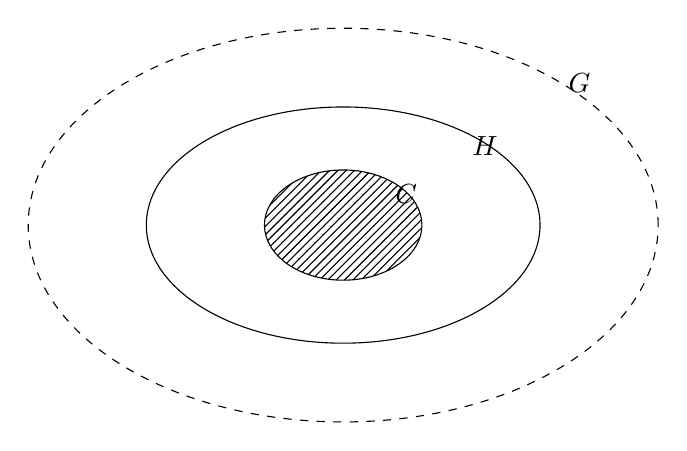
\begin{tikzpicture}
					% Draw the outer dashed ellipse (G)
					\draw[dashed] (0,0) ellipse (4 and 2.5);
					\node at (3, 1.8) {$G$};
					
					% Draw the middle solid ellipse (H)
					\draw (0,0) ellipse (2.5 and 1.5);
					\node at (1.8, 1) {$H$};
					
					% Draw the inner filled and hatched ellipse (C)
					\fill[pattern=north east lines] (0,0) ellipse (1 and 0.7);
					\draw (0,0) ellipse (1 and 0.7);
					\node at (0.8, 0.4) {$C$};
				\end{tikzpicture}
			\end{figure} 
			
			Consequently, if we choose the number \( \varepsilon \) sufficiently small, then \( \text{dist}(x, C) > \varepsilon \) for all \( x \in G - \overline{H} \), and hence
			\[
			v_\varepsilon(x) = 0 \quad \text{for all } x \in G - \overline{H},
			\]
			i.e., \( v_\varepsilon \in C_0^\infty(G) \). Summarizing,
			\[
			\|u - v_\varepsilon\| \leq \|u - v\| + \|v - v_\varepsilon\| < 2\eta,
			\]
			i.e., \( C_0^\infty(G) \) is dense in \( L_2(G) \).
			
			\textbf{Case B}: The open set \( G \) is unbounded. Then, for each \( \eta > 0 \), there is an open ball \( B \) such that
			\[
			\int_{G - H} |u|^2 \, dx < \eta^2,
			\]
			where \( H := G \cap B \) and \( H \neq \emptyset \).
			
			Applying \textbf{Case A} to the nonempty \textit{bounded} open set \( H \), there is a function \( v_\varepsilon \in C_0^\infty(H) \), and hence \( v_\varepsilon \in C_0^\infty(G) \), such that
			\[
			\int_H |u - v_\varepsilon|^2 \, dx < \eta^2.
			\]
			
			Since \( v_\varepsilon = 0 \) on \( G - H \), we get
			\[
			\|u - v_\varepsilon\|^2 = \int_{G - H} |u|^2 \, dx + \int_H |u - v_\varepsilon|^2 \, dx < \eta^2,
			\]
			i.e., \( C_0^\infty(G) \) is dense in \( L_2(G) \).
			\item  Since $ C^{\infty}_{0}(G)\subseteq C(\overline{G})$, it follows directly from $(b)$.
		\end{enumerate}
	\end{solution}
	\begin{problem}
		\textbf{Separability}
		(Proof of Corollary 8 in Section 2.2).
		
		\begin{enumerate}[(a)]
			\item Let \( G = \, [a, b] \, \) be a bounded open interval in \( \mathbb{R} \). Show that \( L_2(G) \) is \textit{separable}.
			\item Let \( G \) be an \textit{unbounded} open interval in \( \mathbb{R} \), e.g., \( G = \mathbb{R} \). Show that \( L_2(G) \) is \textit{separable}.
		\end{enumerate}
		
	\end{problem}
	
	\begin{solution}
		\begin{enumerate}[(a)]
			\item Let \( u \in L_2(G) \) and \( \varepsilon > 0 \) be given. Since$C(\overline{G})$ is dense in $L_{2}(G)$ for any nonempty open set $G\in\mathbb{R^{N}}$, the set \( C[a, b] \) is dense in \( L_2(G) \), i.e., there is a function \( v \in C[a, b] \) such that
			\[
			\|u - v\| = \left( \int_a^b |u - v|^2 \, dx \right)^{\frac{1}{2}} < \varepsilon.
			\]
			
			By the \textit{Weierstrass approximation theorem}, the set of polynomials with real coefficients is dense in the Banach space \( C[a, b] \), i.e., there is a real polynomial \( p \) such that
			\[
			\|v - p\|_* \coloneqq \max_{a \leq x \leq b} |v(x) - p(x)| < \varepsilon.
			\]
			
			Let us introduce
			\[
			\mathcal{M} \coloneqq \text{set of all polynomials with rational coefficients}.
			\]
			
			For each real number $a_{j}$ and each $\varepsilon>0$, there is a rational number $r_{j}$ such that\[ |a_{j} - r_{j}| <\varepsilon \]
			Thus for each polynomial \( p \), there is a polynomial \( q \in \mathcal{M} \) such that
			\[
			\|p - q\|_* < \sum_{j=0}^{n}|a_{j} - r_{j}|(\max_{a \leq x \leq b}|x|)^{j}\leq \text{const}\cdot\varepsilon.
			\]
			
			Hence \( \|v - q\|_* \leq \|v - p\|_* + \|p - q\|_* < 2\varepsilon \). This implies
			\[
			\|v - q\| = \left( \int_a^b |v - q|^2 \, dx \right)^{\frac{1}{2}} \leq (b - a)^{\frac{1}{2}} \|v - q\|_* < (b - a)^{\frac{1}{2}} 2\varepsilon.
			\]
			
			Summarizing, for each \( \varepsilon > 0 \), there is a \( q \in \mathcal{M} \) such that
			\[
			\|u - q\| \leq \|u - v\| + \|v - q\| < \varepsilon + (b - a)^{\frac{1}{2}} 2\varepsilon.
			\]
			
			That is, the set \( \mathcal{M} \) is dense in \( L_2(G) \). Since the set \( \mathcal{M} \) is countable, the space \( L_2(G) \) is \textit{separable}.
			\item  There exists a sequence \( (G_n) \) of \textit{bounded} open intervals in \( G \) such that \( G_1 \subseteq G_2 \subseteq \cdots \subseteq G \) and
			\[
			G = \bigcup_{n=1}^{\infty} G_n.
			\]
			
			Define
			\[
			\chi_n(x) := \begin{cases} 
				1 & \text{if } x \in G_n, \\
				0 & \text{if } x \in \mathbb{R} - G_n,
			\end{cases}
			\]
			and
			\[
			\mathcal{M}_\infty := \{\chi_n q : q \in \mathcal{M} \text{ and } n = 1, 2, \dots \}.
			\]
			Where \[ \chi_nq\coloneqq \chi_{n}(x)\cdot q(x)=\begin{cases}
				q(x) & \text{if } x\in G_{n}\\
				0 & \text{if } x\in \mathbb{R} - G_{n}
 			\end{cases}  \]
			Since $\mathcal{M}$ is countable, it suffices to show $\mathcal{M}$ is dense in $L_{2}(G)$. Let \( u \in L_2(G) \) and \( \varepsilon > 0 \) be given. There exists a \textit{bounded} interval \( J \) with \( J \subseteq G \) and
			\[
			\int_{G - J} |u|^2 \, dx < \varepsilon^2,
			\]
			by a well-known property of the Lebesgue integral. Choose some interval \( G_n \) such that \( J \subseteq G_n \subseteq G \). Then
			\[
			\int_{G - G_n} |u|^2 \, dx \leq \int_{G - J} |u|^2 \, dx < \varepsilon^2.
			\]
			
			By $(a)$, for any bounded set $G_{n}$, there is a polynomial \( q \in \mathcal{M} \) such that
			\[
			\int_{G_n} |u - q|^2 \, dx < \varepsilon^2.
			\]
			
			Hence
			\[
			\|u - \chi_n q\|^2 = \int_{G - G_n} |u|^2 \, dx + \int_{G_n} |u - q|^2 \, dx < 2\varepsilon^2.
			\]
			
			Consequently, the \textit{countable} set \( \mathcal{M}_\infty \) is dense in \( L_2(G) \), i.e., \( L_2(G) \) is \textit{separable}.
			
		\end{enumerate}
	\end{solution}
\end{document}





















-

















































































































